\section{Linear Support Vector Machines} 

  Remember that it was the assumption that the conditional distribution $Y \mid X = x$ being Bernoulli/multinomial, along with the power form of the surrogate likelihood, that led to the likelihood derivation of the surrogate loss of the logistic and softmax regression. But ultimately, these are just modeling assumptions, and we may look for other surrogate losses to construct our risk. 

  If we want to construct such a loss function, we first want it to approximate the $0$-$1$ step function clearly. The next thing is that we want it to be convex, so we can use convex optimization (sum of convex functions are convex). Perhaps we can think of the \textit{smallest} convex function that stays above the binary loss, in some sense the best approximation. This is precisely the hinge function. 

  \begin{definition}[Hinge Loss]
    The \textbf{hinge loss} is a convex surrogate loss function for the 0-1 loss function. It is defined as 
    \begin{equation}
      L(y, \hat{y}) = \max(0, 1 - y \cdot \hat{y})
    \end{equation}
  \end{definition} 

  Note that we have directly constructed a loss without any reference to the likelihood of the data points. Now the SVM model is really simple. We just have a linear model $g(x) = \beta^T x$, and then use it to make a plug-in classifier through a threshold function with threshold $0$. 

  \begin{definition}[Binary Support Vector Machine]
    The \textbf{binary SVM} is a linear classifier that sets 
    \begin{equation}
      f(x) = \mathrm{sign}(F(x)) = \mathrm{sign}(\beta^T x) = \begin{cases} 
        1 & \text{ if } \beta^T x \geq 0 \\
        0 & \text{ else}
      \end{cases}
    \end{equation}
  \end{definition} 

  With the model and loss set up, we can define our risk.

  \begin{theorem}[Risk]
    The expected risk is 
    \begin{equation}
      R(f) = \mathbb{E}_{x, y} \left[ \max\{0, 1 - y F(x) \}\right] = \mathbb{E}_{x, y} \left[ \max\{0, 1 - y (\beta^T x) \}\right]
    \end{equation}
    and the empirical risk is 
    \begin{equation}
      \hat{R}(f) = \frac{1}{n} \sum_{i=1}^n \max\{0, 1 - y (\beta^T x) \}
    \end{equation}
  \end{theorem}
  
  Note that if we classified something correctly, then $y(\beta^T x)$ would be positive, leading to the loss term being cut off to $0$.\footnote{Unless $\beta^T x$ was a very small positive number, but speaking loosely here.} So the model will focus only on the points that are wrong or that are most difficult to tell apart, which are called the \textit{support vectors}. The other points ``far away'' from the decision boundary have little to no effect on the optimal solution, and this is a big difference between SVMs and other classifiers. 

  \begin{example}[SVMs vs Other Classifiers on Linearly Separable Dataset]
    Assume that our dataset $\mathcal{D} = \{\mathbf{x}_i, y_i\}$ is linearly separable with $y_i \in \{-1, +1\}$. Based on previous algorithms like the perceptron, it will find some separating hyperplane. However, there's an infinite number of separating hyperplanes as shown in Figure \ref{fig:svm_intro_1}. What support vector machines want to do is to find the best one, with the ``best" defined as the hyperplane that maximizes the distance between either the closest positive or negative samples, shown in Figure $\ref{fig:svm_intro2}$.  

    \begin{figure}[H] 
      \centering 
      \begin{subfigure}[b]{0.45\textwidth} 
        \centering 
        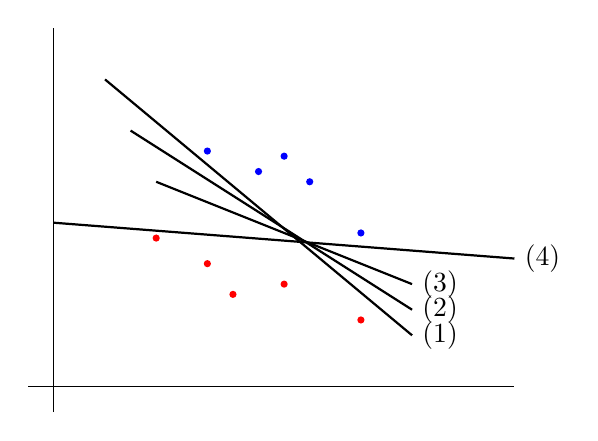
\begin{tikzpicture}[scale=0.65]
          % Draw axes
          \draw[-] (-0.5,0) -- (9,0);
          \draw[-] (0,-0.5) -- (0,7);
          
          % Intersection point
          \coordinate (I) at (4,3);
          
          % Draw numbered lines
          \draw[thick] (1,6) -- (7,1) node[right] {(1)};
          \draw[thick] (1.5,5) -- (7,1.5) node[right] {(2)};
          \draw[thick] (2,4) -- (7,2) node[right] {(3)};
          \draw[thick] (0,3.2) -- (9,2.5) node[right] {(4)};
          
          % Add blue points (above lines)
          \fill[blue] (3,4.6) circle (2pt);
          \fill[blue] (4,4.2) circle (2pt);
          \fill[blue] (5,4) circle (2pt);
          \fill[blue] (6,3) circle (2pt);
          \fill[blue] (4.5,4.5) circle (2pt);
          
          % Add red points (below lines)
          \fill[red] (2,2.9) circle (2pt);
          \fill[red] (3,2.4) circle (2pt);
          \fill[red] (3.5,1.8) circle (2pt);
          \fill[red] (4.5,2) circle (2pt);
          \fill[red] (6,1.3) circle (2pt);
        \end{tikzpicture}
        \caption{Planes such as (1) and (4) are ``too close" to the positive and negative samples. } 
        \label{fig:svm_intro_1}
      \end{subfigure}
      \hfill
      \begin{subfigure}[b]{0.45\textwidth} 
        \centering 
        \begin{tikzpicture}[scale=0.65]
          % Draw axes
          \draw[-] (-0.5,0) -- (9,0);
          \draw[-] (0,-0.5) -- (0,7);
          
          % Intersection point
          \coordinate (I) at (4,3);
          
          % Draw numbered lines
          \draw[thick] (1,5) -- (7,1.5);
          \draw[dotted, thick] (1,5.8) -- (7,2.3);
          \draw[dotted, thick] (1,4.2) -- (7,0.7);
          
          % Add blue points (above lines)
          \fill[blue] (3,4.6) circle (2pt);
          \fill[blue] (4,4.2) circle (2pt);
          \fill[blue] (5,4) circle (2pt);
          \fill[blue] (6,3) circle (2pt);
          \fill[blue] (4.5,4.5) circle (2pt);
          
          % Add red points (below lines)
          \fill[red] (2,2.9) circle (2pt);
          \fill[red] (3,2.4) circle (2pt);
          \fill[red] (3.5,1.8) circle (2pt);
          \fill[red] (4.5,2) circle (2pt);
          \fill[red] (6,1.3) circle (2pt);
        \end{tikzpicture}
        \caption{SVMs try to find the separating hyperplane with the best minimum margin.} 
        \label{fig:svm_intro2}
      \end{subfigure} 
      \caption{Motivating problem} 
      \label{fig:svm_intro} 
    \end{figure}
  \end{example} 

  We want to formalize the concepts of these margins that we wish to maximize. Furthermore, this problem is not well defined since we can just set $w$ to be $0$ or an arbitrarily high norm vector, which makes this problem ill-posed. Therefore, we will need some constraints as well. 

\subsection{Functional and Geometric Margins} 
  
  To do this, we will define two terms. 

  \begin{definition}[Geometric margin]
    Given a point $\mathbf{x}_0$ and a hyperplane of equation $\mathbf{w} \cdot \mathbf{x} + b = 0$, the distance from $\mathbf{x}_0$ to the hyperplane, known as the \textbf{geometric margin}, can be computed with the formula 

    \begin{equation}
      d = \frac{|\mathbf{x}_0 \cdot \mathbf{w} + b|}{||\mathbf{w}||}  
    \end{equation} 

    Therefore, the geometric margin of the $i$th sample with respect to the hypothesis $f$ is defined 

    \begin{equation}
      \gamma_i = \frac{y_i \, (\mathbf{w} \cdot \mathbf{x}_i + b)}{||\mathbf{w}||} 
    \end{equation} 
  \end{definition}

  We wish to optimize the parameters $\mathbf{w}, b$ in order to maximize the minimum of the geometric margins (the distance between the closest point and the hyperplane). 

  \begin{equation}
    \argmax_{\mathbf{w}, b} \min_i \gamma_i = \argmax_{\mathbf{w}, b} \bigg\{ \frac{1}{||\mathbf{w}||} \min_i \big[y_i \, (\mathbf{w} \cdot \mathbf{x}_i + b) \big] \bigg\}
  \end{equation}

  Direct solution of this optimization problem would be very complex, and so we convert this into an equivalent problem that is much easier to solve. Note that the solution to the above term is not unique. If there was a solution $(\mathbf{w}^\ast, b^\ast)$, then 

  \begin{equation}
    \frac{y_i (\mathbf{w} \cdot \mathbf{x}_i + b)}{||\mathbf{w}||} = \frac{y_i (\lambda \mathbf{w} \cdot \mathbf{x}_i + \lambda b)}{||\lambda \mathbf{w}||}  
  \end{equation}

  That is, the geometric margin is not sensitive to scaling of the parameters of the hyperplane. Therefore, we can scale the numerator and the denominator by whatever we want and use this freedom to set 

  \begin{equation*}
    y_i ( \mathbf{w} \cdot \mathbf{x}_i + b ) = 1 
  \end{equation*}
  
  for the point that is closest to the surface. In that case, all data points will satisfy the constraints 

  \begin{equation*}
    y_n (\mathbf{w} \cdot \mathbf{x}_i + b) \geq 1
  \end{equation*}

  In the case of data points for which the equality holds, the constraints are said to be \textit{active}, whereas for the remainder they are \textit{inactive}. Therefore, it will always be the case that $\min_i \big[ y_i \, (\mathbf{w} \cdot \mathbf{x}_i + b)\big] = 1$, and the constraint problem reduces to 

  \begin{equation}
    \argmax_{\mathbf{w}, b} \frac{1}{||\mathbf{w}||} = \argmin_{\mathbf{w}, b} \frac{1}{2} ||\mathbf{w}||^2 \text{ subject to constraints } y_i (\mathbf{w} \cdot \mathbf{x}_i + b) \geq 1 
  \end{equation}

  This final step is the most significant step in this derivation and may be hard to wrap around the first time. So we dedicate the next subsubsection for this. 

  
  We could just work straight with this geometric margin, but for now, let's try to extend what we did with the perceptron into SVMs. We will find out that extending the concept of functional margins into SVMs leads to ill-defined problems. In the perceptron, we wanted to construct a function $f(\mathbf{x}) = \mathbf{w} \cdot \mathbf{x} + b$ such that 
  \begin{equation*}
    y_i \, f(\mathbf{x}_i) \geq 0 \text{ for all } i = 1, 2, \ldots, N
  \end{equation*}

  \begin{definition}[Functional Margin]
    The value of $y_i \, f(\mathbf{x}_i)$ gives us our confidence on our classification, and in a way it represents a kind of distance away from the separating hyperplane (if this value was $0$, then we would be 50 50 split on whether to label it positive or negative). Therefore, we shall define 
    \begin{equation*}
        \hat{\gamma}_i = y_i f(\mathbf{x}_i) 
    \end{equation*}
  as the \textbf{functional margin} of $(\mathbf{w}, b)$ with respect to the training sample $(\mathbf{x}_i, y_i)$. Therefore, the smallest of the function margins can be written 
  \begin{equation*}
      \hat{\gamma} = \min_i \gamma_i 
  \end{equation*}
  called the \textbf{function margin}. 
  \end{definition}

  Note that the geometric margin and functional margin are related by a constant scaling factor. Given a sample $(\mathbf{x}_i, y_i)$, we have 
  \begin{equation*}
      \mathrm{Geometric Margin} = \frac{y_i \, (\mathbf{w} \cdot \mathbf{x}_i + b)}{||\mathbf{w}||_2} = \frac{\mathrm{Functional Margin}}{||\mathbf{w}||_2}
  \end{equation*}

  As we can see, the perceptron works with the functional margin, and since it does not care about how large the margin is (just whether it's positive or negative), we are left with an underdetermined system in which there exists infinite $(\mathbf{w}, b)$'s. Now what we want to do is impose a certain minimum margin $\gamma > 0$ and solve for $(\mathbf{w}, b)$ again, and keep increasing this $\gamma$ until there is some unique solution. We can view this problem in two ways: 
  \begin{enumerate} 
      \item Take a specific minimum margin $\gamma$ and find a $(\mathbf{w}, b)$, which may not exist, be unique, or exist infinitely that satisfies 
          \begin{equation*}
              y_i f(\mathbf{x}) = y_i ( \mathbf{w} \cdot \mathbf{x} + b) \geq \gamma \text{ for all } i = 1, \ldots, N 
          \end{equation*}
      \item Take a specific $(\mathbf{w}, b)$ and calculate the maximum $\gamma$ that satisfies the constraint equations above.  
  \end{enumerate}

  They're both equivalent problems, but both ill-posed if we look at (2). Since the samples are linearly separable by assumption, we can say that there exists some $\epsilon > 0$ such that $y_i f(\mathbf{x}_i) \geq \epsilon$ for all $i$. Therefore, if we just scale $(\mathbf{w}, b) \mapsto (\lambda \mathbf{w}, \lambda b)$ for some large $\lambda$, this leads to the solution for $\gamma$ being unbounded. We can see in Figure $\ref{fig:scaling_problem}$ that we can increased confidence at no cost. Looking at (1), we can also see that if $(\mathbf{w}, b)$ does exist, then every other $(\lambda \mathbf{w}, \lambda b)$ for $\lambda > 1$ satisfies the property.   

  \begin{figure}[H] 
    \centering 
    \begin{subfigure}[b]{0.32\textwidth} 
      \centering 
      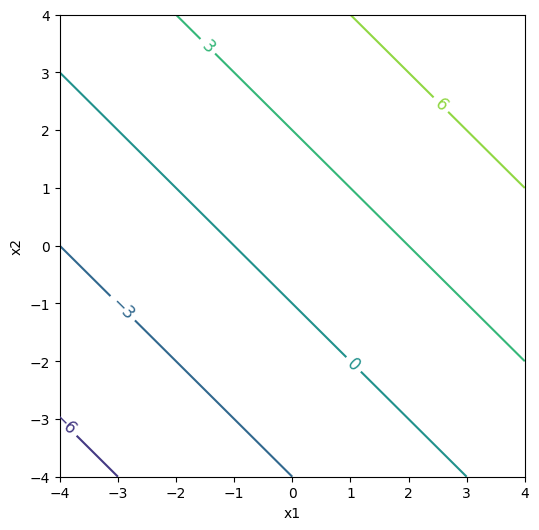
\includegraphics[width=\textwidth]{img/scaling1.png} 
      \caption{$f(x) = x_1 + x_2 + 1$} 
      \label{fig:original_scaled}
    \end{subfigure} 
    \hfill    
    \begin{subfigure}[b]{0.32\textwidth} 
      \centering 
      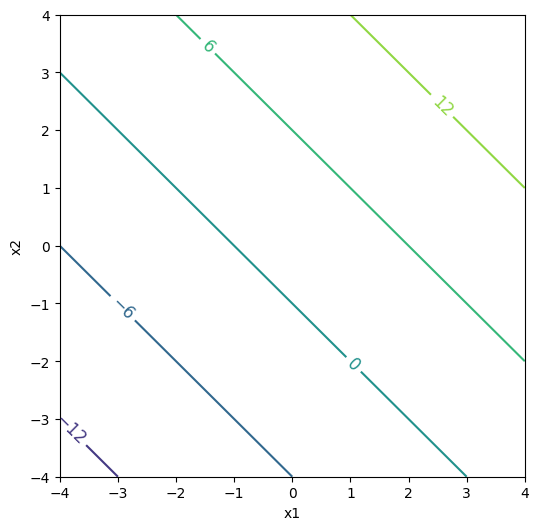
\includegraphics[width=\textwidth]{img/scaling2.png} 
      \caption{$f(x) = 2 x_1 + 2 x_2 + 2$} 
      \label{fig:two_times_scaled}
    \end{subfigure} 
    \hfill
    \begin{subfigure}[b]{0.32\textwidth} 
      \centering 
      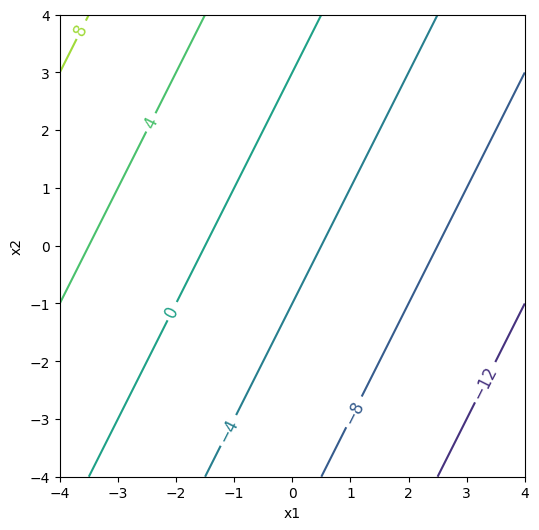
\includegraphics[width=\textwidth]{img/scaling3.png} 
      \caption{$f(x) = -2x_1 + x_2 - 3$} 
      \label{fig:something_else}
    \end{subfigure} 
    \caption{From (a), you can see that simply multiplying everything by two automatically increases our confidence by $2$, meaning that the functional margin can be scaled arbitrarily by scaing $(\mathbf{w}, b)$. There are still too many degrees of freedom in here and so extra constraints must be imposed. } 
    \label{fig:scaling_problem} 
  \end{figure}

\subsection{Analytical Solution} 

  To minimize the equations with the constraint equations, we can use the method of Lagrange multipliers, which leads to to Lagrangian 
  \[\mathcal{L}(\mathbf{w}, b, \boldsymbol{\alpha}) = \frac{1}{2} ||\mathbf{w}||^2 - \sum_i \alpha_i \big[ y_i (\mathbf{w} \cdot \mathbf{x}_i + b) - 1\big]\]
  We can take the gradients with respect to $\mathbf{w}$ and $b$ and set them to $0$, which gives the two conditions 
  \begin{align*} 
    \mathbf{w} & = \sum_i \alpha_i y_i \mathbf{x}_i \\
    0 & = \sum_i \alpha_i y_i \mathbf{x}_i 
  \end{align*}

  Now let's substitute our evaluated $\mathbf{w}$ back into $\mathcal{L}$, which gives the \textbf{dual representation} of the maximum margin problem in which we maximize  
  \begin{align*} 
      L & = \frac{1}{2} \bigg( \sum_i \alpha_i y_i \mathbf{x}_i \bigg) \bigg( \sum_j \alpha_j y_j \mathbf{x}_j \bigg) - \sum_{i} \alpha_i y_i x_i \cdot \bigg[ \sum_j \alpha_j y_j x_j \bigg] - \sum_i \alpha_i y_i b + \sum_i \alpha_i \\ 
        & = \sum_i \alpha_i - \frac{1}{2} \sum_{i, j} \alpha_i \alpha_j y_i y_j \, \mathbf{x}_i \cdot \mathbf{x}_j 
  \end{align*}
  The summation with the $b$ in it is $0$ since we can pull the $b$ out and the remaining sum is $0$ from before. Now the optimization only depends on the dot product $\mathbf{x}_i \cdot \mathbf{x}_j$ of all pairs of sample vectors, which is very interesting. We will see more of this when we talk about kernel methods. Now, we need to solve the dual problem 
  \[\max_{\boldsymbol{\alpha}} \mathcal{L}(\boldsymbol{\alpha})\]
  which can be done using some generic quadratic programming solver or some other method to get the optimum $\boldsymbol{\alpha}^\ast$, which gives us 
  \[\mathbf{w}^\ast = \sum_i \alpha_i^\ast y_i \mathbf{x}_i\]

\subsection{Significance Tests and Confidence Sets}

\subsection{Concentration Bounds} 

\subsection{Nonseparable Case} 

